\documentclass[border=15pt, tikz, multi=tikzpicture]{standalone}
\usetikzlibrary{positioning, arrows.meta, fit, backgrounds, calc}

\begin{document}

% ─── Figure 1: Topology — two operators, two relay paths ────────────────────
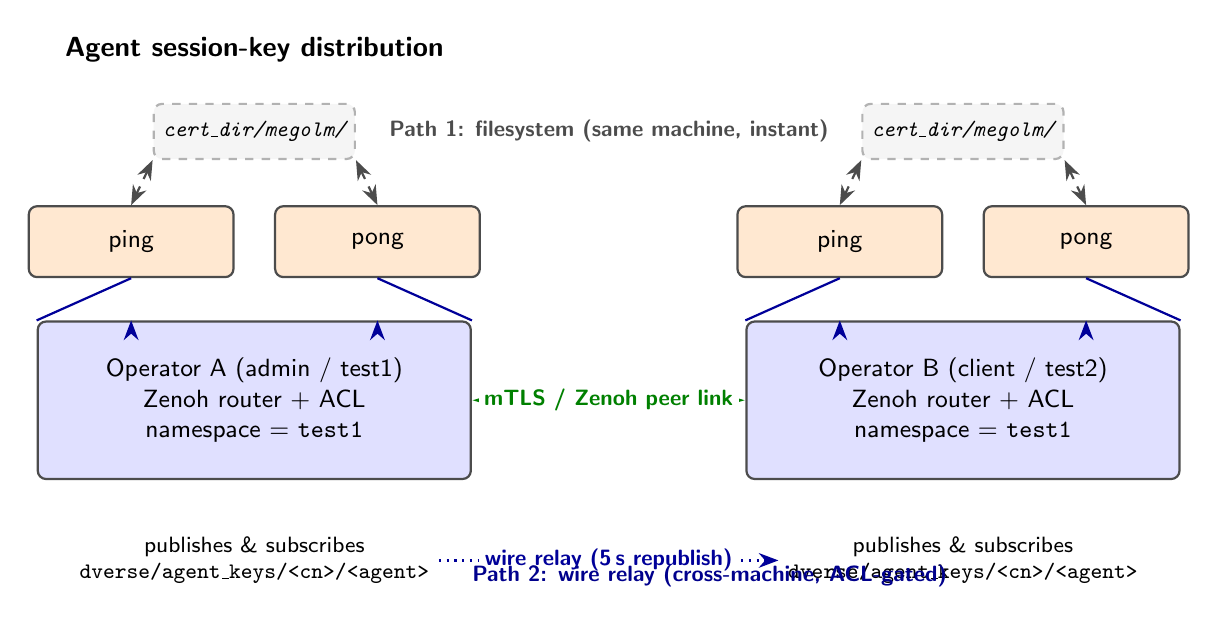
\begin{tikzpicture}[
    node distance=0.5cm,
    agent/.style={
      rectangle, draw=black!70, thick, rounded corners=3pt,
      fill=orange!18, font=\small\sffamily, align=center,
      minimum width=2.6cm, minimum height=0.9cm,
    },
    router/.style={
      rectangle, draw=black!70, thick, rounded corners=3pt,
      fill=blue!12, font=\small\sffamily, align=center,
      minimum width=5.5cm, minimum height=2cm,
    },
    fsbus/.style={
      rectangle, draw=gray!60, thick, dashed, rounded corners=3pt,
      fill=gray!8, font=\footnotesize\sffamily\itshape, align=center,
      minimum width=2.2cm, minimum height=0.7cm,
    },
    label/.style={font=\footnotesize\sffamily, align=center},
    wirelabel/.style={
      font=\footnotesize\sffamily\bfseries,
      fill=white, inner sep=2pt,
    },
    fslabel/.style={font=\footnotesize\sffamily\itshape, fill=white, inner sep=2pt},
    msg/.style={-{Stealth[length=2.5mm]}, thick, blue!60!black},
    fs/.style={{Stealth[length=2.5mm]}-{Stealth[length=2.5mm]}, thick, dashed, gray!60!black},
    mesh/.style={{Latex[length=2.2mm]}-{Latex[length=2.2mm]}, thick, green!50!black},
]

% Two operators
\node[router] (opA) at (0, 0)   {Operator A (admin / test1)\\Zenoh router + ACL\\namespace = \texttt{test1}};
\node[router] (opB) at (9, 0)   {Operator B (client / test2)\\Zenoh router + ACL\\namespace = \texttt{test1}};

% Agents on top of each operator
\node[agent] (pingA) at ($(opA.north west)+(1.2,1.0)$) {ping};
\node[agent] (pongA) at ($(opA.north east)+(-1.2,1.0)$) {pong};
\node[agent] (pingB) at ($(opB.north west)+(1.2,1.0)$) {ping};
\node[agent] (pongB) at ($(opB.north east)+(-1.2,1.0)$) {pong};

% Same-machine filesystem bus
\node[fsbus] (fsA) at ($(opA.north)+(0,2.4)$) {\texttt{cert\_dir/megolm/}};
\node[fsbus] (fsB) at ($(opB.north)+(0,2.4)$) {\texttt{cert\_dir/megolm/}};

% FS arrows (same-machine, instant)
\draw[fs] (pingA.north) -- (fsA.south west);
\draw[fs] (pongA.north) -- (fsA.south east);
\draw[fs] (pingB.north) -- (fsB.south west);
\draw[fs] (pongB.north) -- (fsB.south east);

% Agents → their operator (carries published agent_keys + payloads)
\draw[msg] (pingA.south) -- (opA.north west) ++(1.2,0);
\draw[msg] (pongA.south) -- (opA.north east) ++(-1.2,0);
\draw[msg] (pingB.south) -- (opB.north west) ++(1.2,0);
\draw[msg] (pongB.south) -- (opB.north east) ++(-1.2,0);

% Inter-router TLS mesh
\draw[mesh] (opA.east) -- node[wirelabel] {mTLS / Zenoh peer link} (opB.west);

% Wire-relay arrow underneath the routers
\node[label, below=0.6cm of opA] (relayA) {publishes \& subscribes\\\texttt{dverse/agent\_keys/<cn>/<agent>}};
\node[label, below=0.6cm of opB] (relayB) {publishes \& subscribes\\\texttt{dverse/agent\_keys/<cn>/<agent>}};
\draw[msg, dotted] (relayA) -- node[wirelabel] {wire relay (5\,s republish)} (relayB);

% Side labels for the two key-distribution channels
\node[font=\footnotesize\sffamily\bfseries, text=gray!60!black, anchor=west]
    at ($(fsA.east)+(0.3,0)$) {\itshape Path 1: filesystem (same machine, instant)};
\node[font=\footnotesize\sffamily\bfseries, text=blue!55!black, anchor=west]
    at ($(relayA.east)+(0.3,-0.2)$) {\itshape Path 2: wire relay (cross-machine, ACL-gated)};

% Title
\node[font=\sffamily\bfseries, above=0.4cm of fsA] {Agent session-key distribution};
\end{tikzpicture}


% ─── Figure 2: Sequence — peer-key install across operators ──────────────────
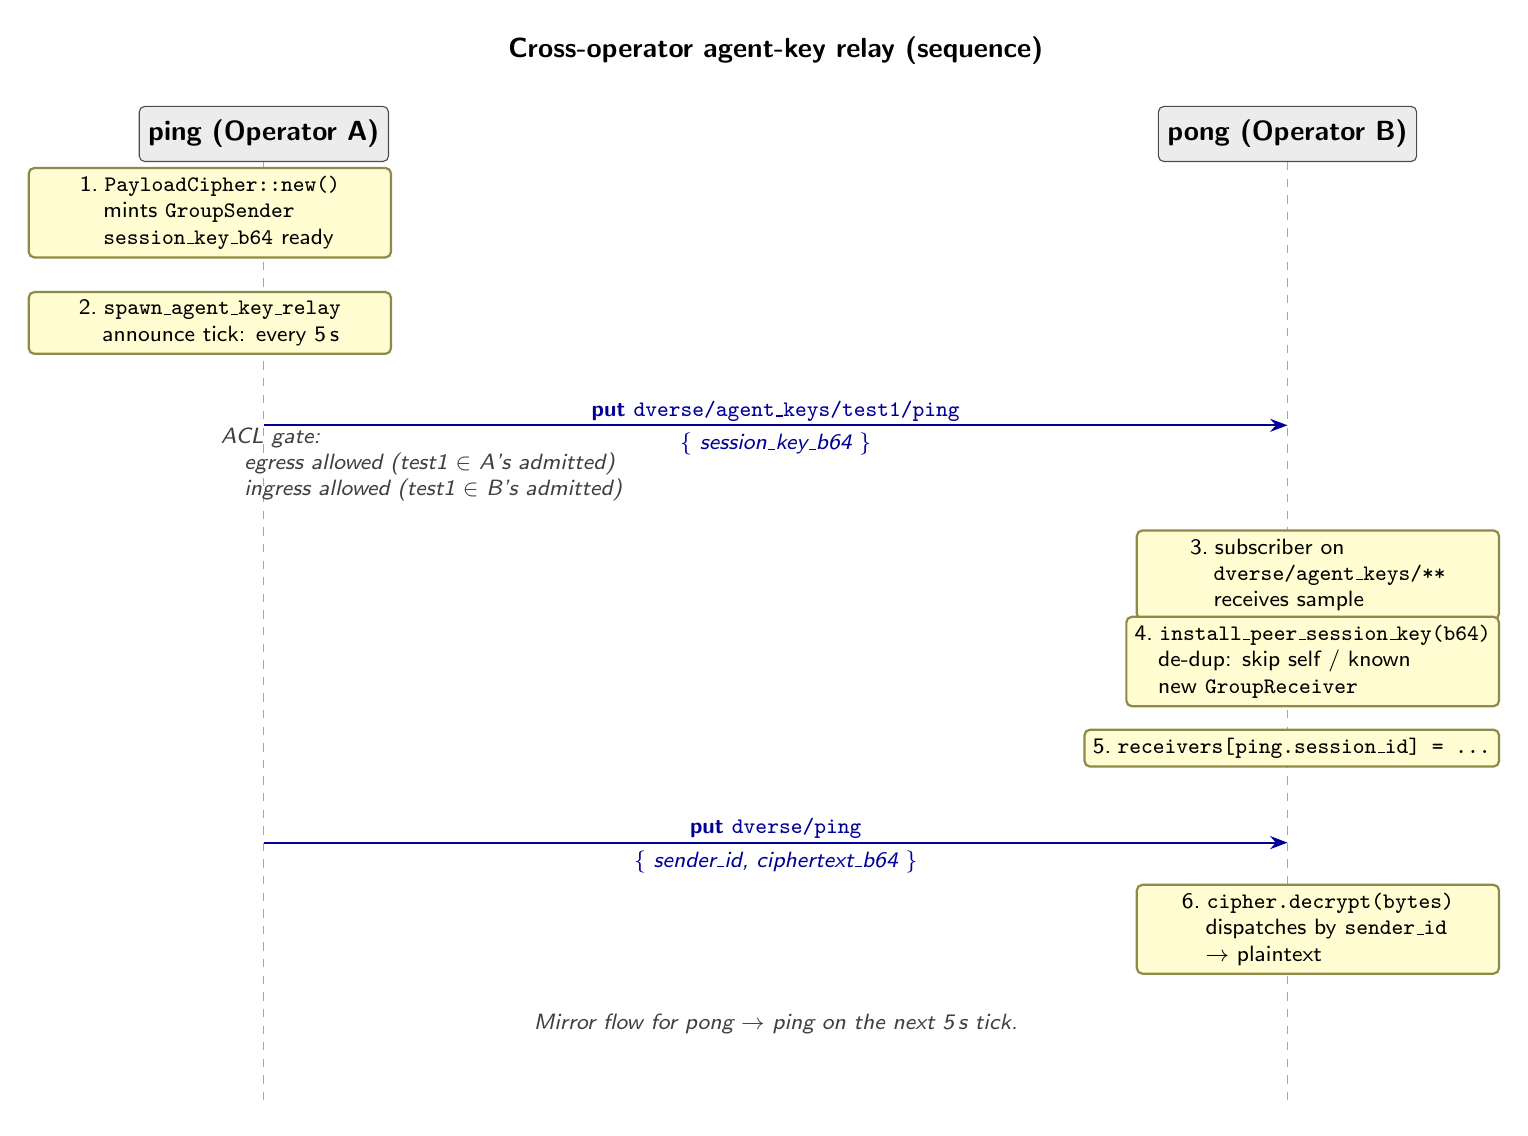
\begin{tikzpicture}[
    actor/.style={
      font=\sffamily\bfseries, align=center,
      draw=black!70, fill=gray!15, rectangle, rounded corners=2pt,
      minimum width=3cm, minimum height=0.7cm,
    },
    action/.style={
      font=\footnotesize\sffamily, anchor=west,
      fill=yellow!18, draw=yellow!50!black, thick,
      rectangle, rounded corners=2pt, inner sep=3pt,
      minimum width=4.6cm, align=left,
    },
    actionR/.style={action, anchor=east},
    msg/.style={-{Stealth[length=2.2mm]}, thick, blue!60!black},
    msglabel/.style={
      font=\footnotesize\sffamily\bfseries, midway, above,
      fill=white, inner sep=1pt,
    },
    msgpayload/.style={
      font=\footnotesize\sffamily\itshape, midway, below=0.5mm,
      fill=white, inner sep=1pt,
    },
    life/.style={dashed, gray!70},
    note/.style={
      font=\footnotesize\sffamily\itshape, text=gray!50!black,
      anchor=west, align=left,
    },
]
% Actors
\node[actor] (P) at (0, 0)  {ping (Operator A)};
\node[actor] (Q) at (13, 0) {pong (Operator B)};

% Lifelines
\draw[life] (P.south) -- ++(0,-12);
\draw[life] (Q.south) -- ++(0,-12);

% ping side: mint sender
\node[action] at (-3, -1.0) {1.\;\texttt{PayloadCipher::new()} \\
                              \quad mints \texttt{GroupSender}\\
                              \quad \texttt{session\_key\_b64} ready};

% ping side: kick off relay
\node[action] at (-3, -2.4) {2.\;\texttt{spawn\_agent\_key\_relay} \\
                              \quad announce tick: every 5\,s};

% Message: agent_keys put
\draw[msg] (P |- 0,-3.7) -- (Q |- 0,-3.7)
    node[msglabel] {put \texttt{dverse/agent\_keys/test1/ping}}
    node[msgpayload] {\{ session\_key\_b64 \}};

% ACL gate (annotation)
\node[note, below=-0.05cm of P, xshift=2cm, yshift=-3.3cm] {
    ACL gate: \\
    \quad egress allowed (test1 $\in$ A's admitted)\\
    \quad ingress allowed (test1 $\in$ B's admitted)
};

% pong side: subscriber path
\node[actionR] at (15.7, -5.6) {3.\;subscriber on \\
                                  \quad \texttt{dverse/agent\_keys/**} \\
                                  \quad receives sample};
\node[actionR] at (15.7, -6.7) {4.\;\texttt{install\_peer\_session\_key(b64)}\\
                                  \quad de-dup: skip self / known\\
                                  \quad new \texttt{GroupReceiver}};
\node[actionR] at (15.7, -7.8) {5.\;\texttt{receivers[ping.session\_id] = …}};

% Now ping encrypts and pong decrypts
\draw[msg] (P |- 0,-9.0) -- (Q |- 0,-9.0)
    node[msglabel] {put \texttt{dverse/ping}}
    node[msgpayload] {\{ sender\_id, ciphertext\_b64 \}};

\node[actionR] at (15.7, -10.1) {6.\;\texttt{cipher.decrypt(bytes)} \\
                                   \quad dispatches by \texttt{sender\_id}\\
                                   \quad $\to$ plaintext};

\node[font=\footnotesize\sffamily\itshape, text=gray!50!black, anchor=center]
    at (6.5, -11.3) {
    Mirror flow for pong $\to$ ping on the next 5\,s tick.
};

\node[font=\sffamily\bfseries, above=0.4cm of P, xshift=6.5cm]
    {Cross-operator agent-key relay (sequence)};
\end{tikzpicture}

\end{document}
